\section{Git remotes}
\begin{frame}[fragile]
  \slidetitle
  This section covers the following topics:
  \begin{itemize}
    \item Git remote repository concept
    \item Working with remotes and forks
    \item Colaborate on a Git repository
  \end{itemize}
\end{frame}

\subsection{Remote repositories}
\begin{frame}[fragile]
  \subslidetitle
  Git has the concept of \textit{remote repositories},
  which are just clones of the same repository located
  somewhere else. \\

  The simplest case of a remote is the \textbf{origin},
  created with a \cmd{git clone}:

  \vspace{3em}
  \centerline{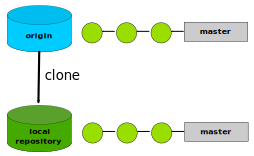
\includegraphics{assets/diagrams/remote-concept.pdf}}
\end{frame}

\subsection{Show remotes}
\begin{frame}[fragile]
  \subslidetitle
  We can use the \cmd{git remote show} command to have a look at the configured remotes:
  \begin{lstlisting}
$ (*\textcolor[HTML]{0000AA}{git remote show}*)
origin

$ (*\textcolor[HTML]{0000AA}{git remote show origin}*)
* remote origin
  Fetch URL: https://github.com/segfault-trainings/gitmoon.git
  Push  URL: https://github.com/segfault-trainings/gitmoon.git
  HEAD branch: master
  Remote branch:
    master tracked
  Local branch configured for 'git pull':
    master merges with remote master
  Local ref configured for 'git push':
    master pushes to master (up to date)
\end{lstlisting}
\end{frame}

\subsection{Forking Workflow}
\begin{frame}[fragile]
  \subslidetitle

  Now let's get our hands dirty in Open Source! \\
  \vspace{1em}

  Our goal is to:
  \begin{itemize}
    \item Use the \textit{Forking Workflow}
    \item Contribute a change to a repository on \href{https://github.com}{GitHub}
  \end{itemize}

  \centerline{\includegraphics[width=\textwidth]{../assets/images/agile-ipsum.jpeg}}

\end{frame}

\subsection{Forking Workflow}
\begin{frame}[fragile]
  \subslidetitle
  Forking Workflow
    \centerline{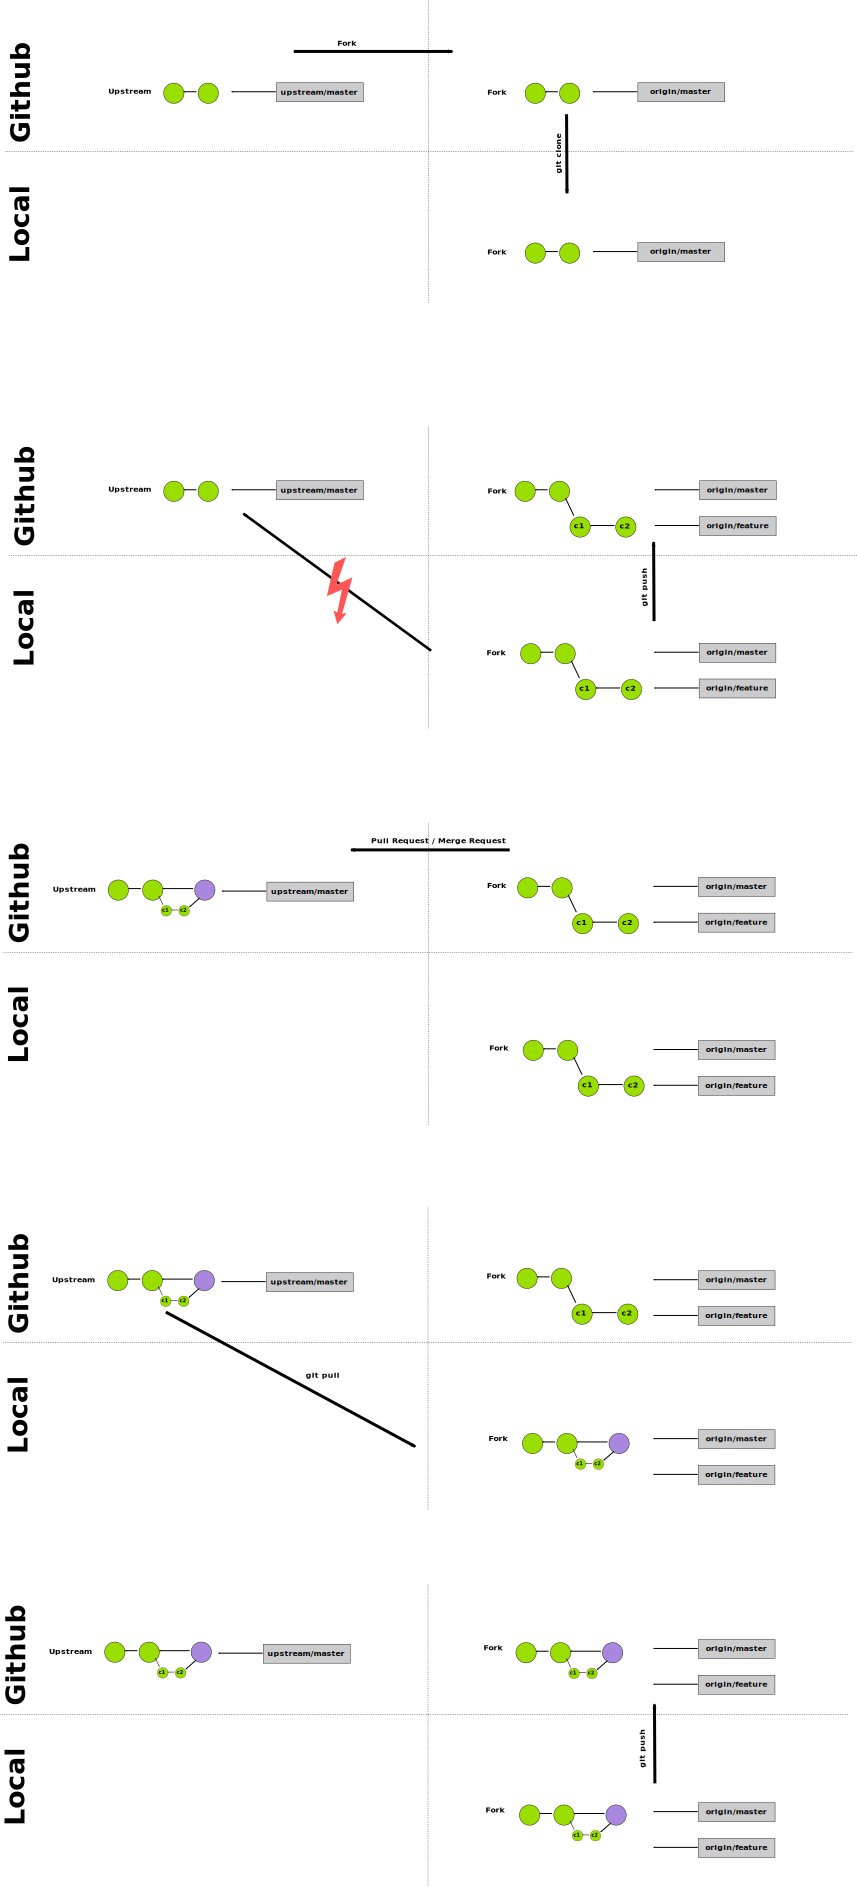
\includegraphics{assets/diagrams/git-forking-workflow.pdf}}

  \vspace{2em}
  \begin{itemize}
    \item Every contributor has it's own copy (fork) of the repo
    \item Contribute with Pull Requests
    \item Most often used in Open Source
  \end{itemize}

\end{frame}

\subsection{Forking Workflow - Fork}
\begin{frame}[fragile]
  \subslidetitle

  Let's create a Fork from our friends awesome \textbf{agile-ipsum} project using \href{https://github.com}{GitHub}:

    \vspace{2em}
    \centerline{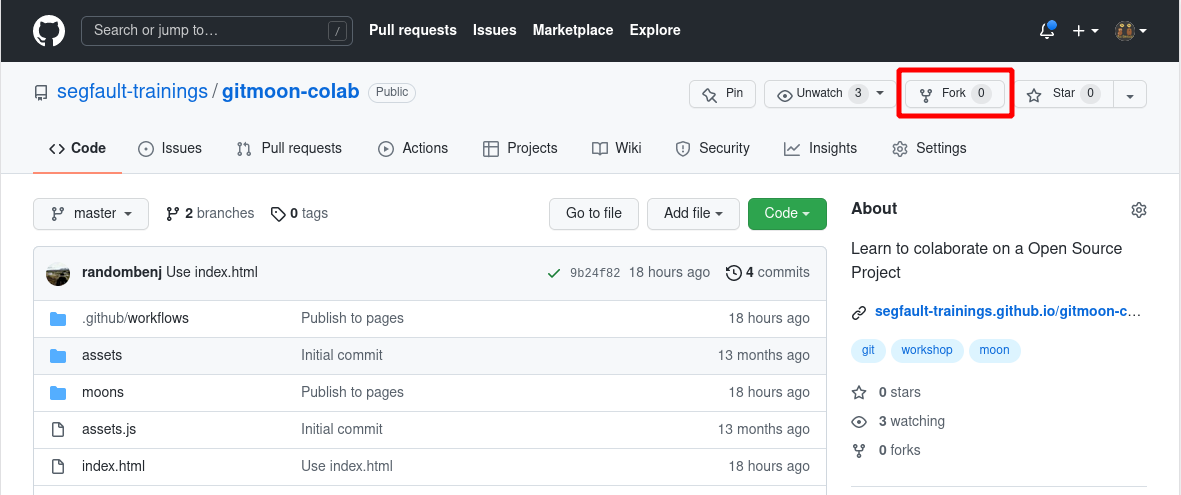
\includegraphics[width=\textwidth]{../assets/images/github-forking.png}}

    \vspace{1em}
  Note: the repository is at \url{https://github.com/BrunnerLivio/agile-ipsum}.

\end{frame}

\subsection{Forking Workflow - Clone}
\begin{frame}[fragile]
  \subslidetitle

    First, we need to \cmd{git clone} our forked repository from the URL provided by GitHub:

    \vspace{1em}
    \centerline{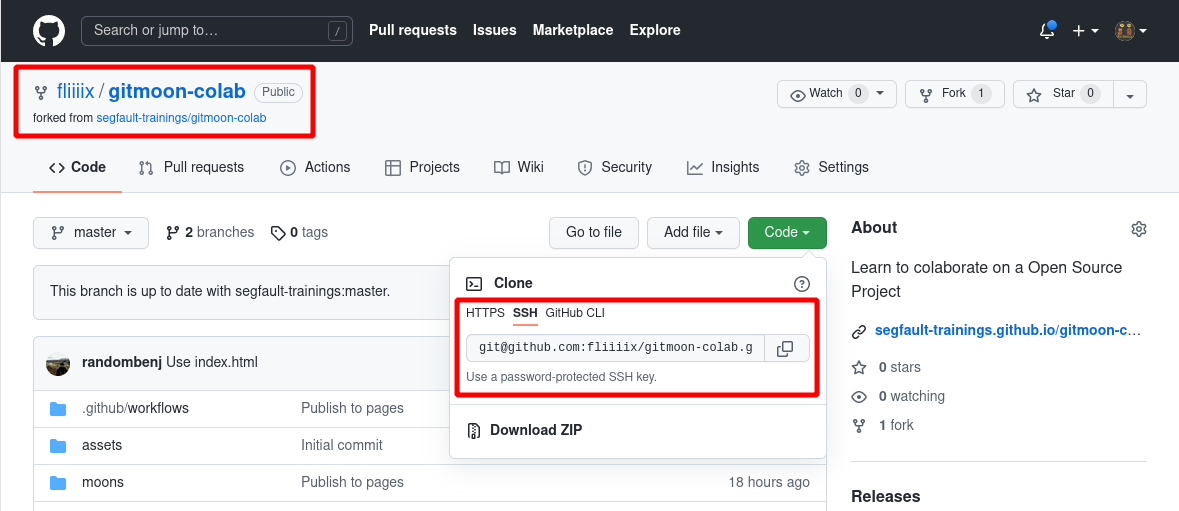
\includegraphics[width=\textwidth]{../assets/images/github-clone.png}}

    \vspace{1em}
    Note: Use HTTPS if you haven't setup an SSH key in your GitHub account for now.
\end{frame}

\subsection{Forking Workflow - Clone}
\begin{frame}[fragile]
  \subslidetitle

  For the next step you should be outside the gitmoon project folder.

  \begin{lstlisting}
$ cd ~
$ (*\textcolor[HTML]{0000AA}{git clone https://github.com/<YOUR USERNAME>/agile-ipsum.git}*)
...

$ (*\textcolor[HTML]{0000AA}{git remote show origin}*)
* remote origin
  Fetch URL: https://github.com/<YOUR USERNAME>/agile-ipsum.git
  Push  URL: https://github.com/<YOUR USERNAME>/agile-ipsum.git
  HEAD branch: master

$ cd agile-ipsum
\end{lstlisting}

\end{frame}

\subsection{Forking Workflow - Change}
\begin{frame}[fragile]
  \subslidetitle

  Let's contribute an \textit{agile term} to the \lstinline{content/dict.js} file.
  \vspace{1em}

  First we'll create a new feature branch:

  \begin{lstlisting}
$ (*\textcolor[HTML]{0000AA}{git switch -c feature/add-new-term}*)
Switched to a new branch 'feature/add-new-term'
\end{lstlisting}

  Second, we make a change to \lstinline{content/dict.js} and create a new commit:

  \begin{lstlisting}
$ (*\textcolor[HTML]{0000AA}{git commit -a -m "Add term XYZ to dict"}*)
[feature/add-new-term 4ab6f8c] Add term XYZ to dict
 1 file changed, 1 insertions(+), 1 deletions(-)
\end{lstlisting}

\end{frame}

\subsection{Forking Workflow - Push}
\begin{frame}[fragile]
  \subslidetitle

  Let's \textit{push} the new branch and it's commits to our fork on GitHub using \cmd{git push}:

  \begin{lstlisting}
$ (*\textcolor[HTML]{0000AA}{git push --set-upstream origin feature/add-new-term}*)
...
To https://github.com/<YOUR USERNAME>/agile-ipsum.git
   6275110..4ab6f8c  feature/add-new-term -> feature/add-new-term
\end{lstlisting}

  \centerline{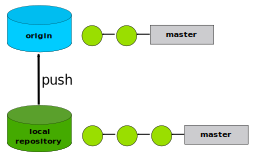
\includegraphics{assets/diagrams/remote-push.pdf}}

\end{frame}

\subsection{Forking Workflow - Pull Request}
\begin{frame}[fragile]
  \subslidetitle

  This change is so valuable that we should contribute it back to the original repository.

  \vspace{1em}
    GitHub uses \textbf{Pull Requests (PR)} for that! Let's create one:

  \vspace{1em}
  \centerline{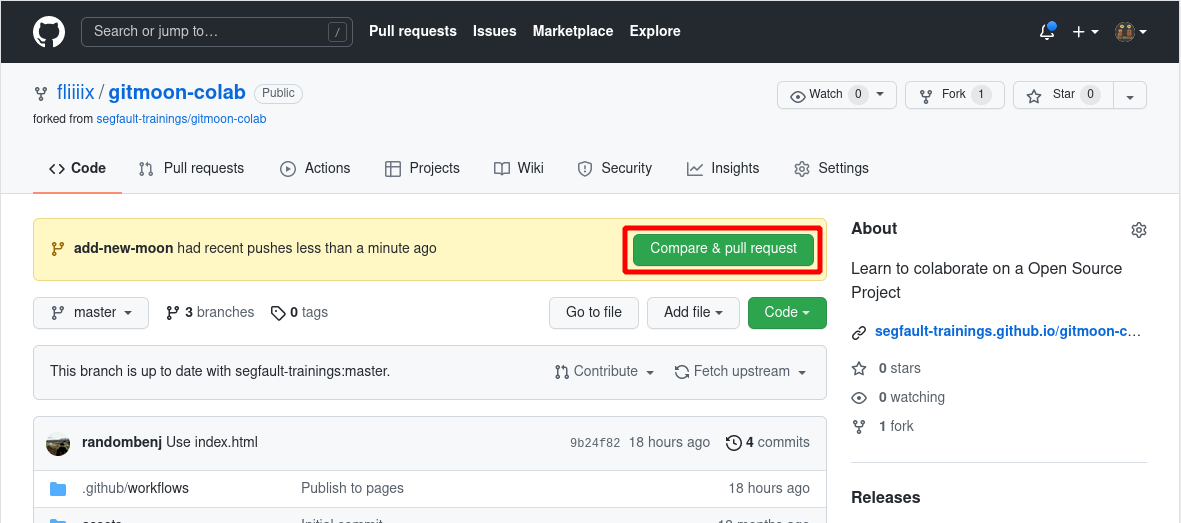
\includegraphics[width=\textwidth]{../assets/images/github-pull-request-create.png}}

\end{frame}

\subsection{Forking Workflow - Pull Request}
\begin{frame}[fragile]
  \subslidetitle

  Always provide a good PR title and description!

  \vspace{1em}
  \centerline{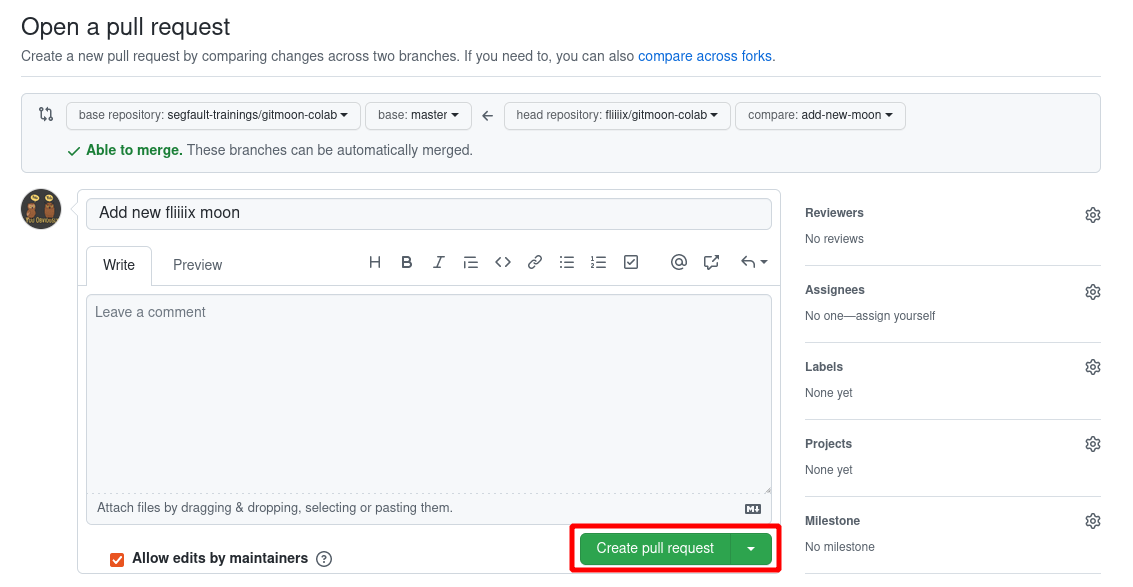
\includegraphics[width=\textwidth]{../assets/images/github-pull-request-submit.png}}

\end{frame}

\subsection{Forking Workflow - Pull Request}
\begin{frame}[fragile]
  \subslidetitle

  \vspace{8em}
  \begin{center}
  Let's wait a little for the maintainer to review and merge those PR!
  \end{center}

\end{frame}

\subsection{Forking Workflow - Upstream}
\begin{frame}[fragile]
  \subslidetitle

  Now your fork is missing all the awesome commits your colleagues made.

  \vspace{2em}
  \centerline{\includegraphics{assets/diagrams/remote-forking-situation.pdf}}

\end{frame}

\subsection{Forking Workflow - Upstream}
\begin{frame}[fragile]
  \subslidetitle

  We want those tasty commits from our colleagues in our fork, too!

  We've seen that our clone only knows the origin remote pointing to our fork:

  \begin{lstlisting}
$ (*\textcolor[HTML]{0000AA}{git remote show}*)
origin
\end{lstlisting}

  To pull those changes, we need to configure a second \textbf{upstream} remote
  to connect our clone to the repository we forked from:

  \begin{lstlisting}
$ (*\textcolor[HTML]{0000AA}{git remote add upstream https://github.com/BrunnerLivio/agile-ipsum}*)

$ (*\textcolor[HTML]{0000AA}{git remote show}*)
origin
upstream
\end{lstlisting}

\end{frame}

\subsection{Forking Workflow - Upstream}
\begin{frame}[fragile]
  \subslidetitle

  Our clone is now connected to two remotes: \textit{origin} and \textit{upstream}:

  \vspace{3em}
  \centerline{\includegraphics{assets/diagrams/remote-concept-with-upstream.pdf}}

  \vspace{1em}
  Note: We can only push to \textit{origin}, but not the \textit{upstream}, because
  we don't have permission to do so.

\end{frame}

\subsection{Forking Workflow - Rebase}
\begin{frame}[fragile]
  \subslidetitle

  Let's fetch the latest changes from the \textit{upstream} remote:

  \begin{lstlisting}
$ (*\textcolor[HTML]{0000AA}{git fetch upstream}*)
\end{lstlisting}

  We can inspect the branches available on upstream:

  \begin{lstlisting}
$ (*\textcolor[HTML]{0000AA}{git branch --remote}*)
origin/master
...
upstream/master
\end{lstlisting}

  And rebase the local \lstinline{master} to the \lstinline{upstream/master} branch:

  \begin{lstlisting}
$ (*\textcolor[HTML]{0000AA}{git switch master}*)
$ (*\textcolor[HTML]{0000AA}{git rebase upstream/master}*)
\end{lstlisting}

  Let's also update our fork on GitHub:

  \begin{lstlisting}
$ (*\textcolor[HTML]{0000AA}{git push}*)
\end{lstlisting}

\end{frame}

\subsection{Forking Workflow - Profit \includegraphics[height=1em]{../assets/images/party-popper_1f389.png}}
\begin{frame}[fragile]
  \subslidetitle

  \vspace{8em}
  \begin{center}
      We successfully contributed to an awesome Open Source project! \includegraphics[height=1em]{../assets/images/party-popper_1f389.png}
  \end{center}

\end{frame}

\subsection{Summary}
\begin{frame}[fragile]
\subslidetitle
  What we've learned in this chapter:
  \begin{itemize}
    \item What remotes are
    \item How to work with remotes
    \item How to apply the Forking Workflow in practice
  \end{itemize}
\end{frame}
